\chapter{Priming neural machine translation}
\label{chap:priming}
This chapter draws from the following publication: \citet{Pham20Priming}
\section{Motivation}
In this chapter, we propose a novel method for non-domain-deterministic testing problem in domain adaptation. This situation require the NMT system adapting to a latent domain of the test sentence on the fly. We are inspired by the idea of \citet{Li18onesentence, Farajian17multidomain}, which used similar sentences to adapt the NMT system to the test sentence. The authors proposed finetuning the NMT model over a batch of similar sentences retrieved from a translation memory. However, we find finetuning the model for each test sentence extremely expensive. Therefore, we propose a novel NMT model, which incorporates the information of retrieved translations to the translation. Our approach relies on a psychology phenomenon called "Priming". 

%Priming is a well known and studied psychology phenomenon based on the prior presentation of one stimulus (cue) to influence the processing of a response. In this work, we propose a framework to mimic the process of priming in the context of neural machine translation (NMT). We evaluate the effect of using similar translations as priming cues on the NMT network. We propose a method to inject priming cues into the NMT network and compare our framework to other mechanisms that perform micro-adaptation during inference. Overall, experiments conducted in a multi-domain setting confirm that adding priming cues in the NMT decoder can go a long way towards improving the translation accuracy. Besides, we show the suitability of our framework to gather valuable information for an NMT network from monolingual resources. 

Priming is a well studied human cognitive phenomenon, founded on the establishment of associations between a stimulus and a response~\cite{Tulving82Priming}. Multiple studies have shown how external stimuli (cues) may have a profound effect on perception.
%
In the case of language translation, external stimuli having such effects are said to prime language understanding and potentially have a impact the actions of a human translator. Imagine for instance a translator facing the ambiguous sentence {\it I was in the bank}, and the effect on translation accuracy if primed with the cue {\it river}. Most likely, the human translator would consider the ``edge of river" sense rather than ``financial institution" for translation. In the context of human translation, cross-lingual priming is particularly effective as cues in the target language may notably influence the final translation word choice.

Several research works have introduced the priming analogy in deep neural networks. In computer vision priming has been broadly studied: for instance, in~\citet{Rosenfeld18Priming}, the authors introduce a cue about the presence of a certain class of object in an image that significantly improves object detection performance. Concerning language generation, \citet{Brown20language}~use a combination of prompt and example to guide the GPT-3 network when performing a task, where the prompt is a sentence that describes the task ({\it i.e. ``Translate from English to French"}); and is followed by an example of the task ({\it i.e. ``sea otter $\leadsto$ loutre de mer"}). In the context of NMT, experiments reported~\cite{Sennrich16politeness,Kobus17domain,dinu19training} aim at influencing translation inference with respectively politeness, domain and terminology constraints. More related to our work,~\cite{bulte19neural,xu20boosting} introduce a simple and elegant framework where similar translations (cues) are used to prime an NMT model, effectively boosting translation accuracy.
In all cases, priming is performed by injecting cues in the input stream prior to inference decoding.

In this work, we extend a framework that mimics the priming process in neural networks, in the context of machine translation. Following up on previous work~\cite{bulte19neural,xu20boosting}, we consider similar translations as external cues that can influence the translation process. We push this concept further:
a) by proposing a novel scheme to integrate similar translation cues into the NMT network. We examine the attention mechanism of the network and confirm that priming stimuli are actually taken into account;
b) by extending an efficient network to train distributed representations of sentences
that are used to identify accurate translations used as priming cues\footnote{\url{https://github.com/jmcrego/cbon}}; 
c) by analyzing how on-the-fly priming compares to micro-adaptation (fine-tuning). 
%
Finally, we show that our priming approach can also be used with monolingual data, providing a scenario where NMT can be effectively helped by large amounts of available data.
%
Our proposal does not require to change the NMT architectures or algorithms, relying solely on input preprocessing and on prefix (forced) decoding \cite{santy19inmt,rebecca16neural}, a feature already implemented in many NMT toolkits.

The remainder of the chapter is organized as follows: Section~\ref{sec:priming-chap8} gives details regarding our priming approach. The experimental framework is presented in Section~\ref{sec:eperiments-chap8}. Results and discussion are respectively in Sections~\ref{sec:results-chap8} and~\ref{sec:discussion-chap8}. We review related work in Section~\ref{sec:related-chap8} and conclude in Section~\ref{sec:conclusions-chap8}.

\section{NMT Priming On-the-fly}
\label{sec:priming-chap8}

This section describes our framework for priming neural MT with similar translations. 
We follow the work by ~\cite{bulte19neural,xu20boosting} and build a translation model that incorporates similar translations from a translation memory (TM) to boost translation accuracy. In this work, TMs are parallel corpora containing translations falling in the same domain as test sentences.

We first describe the methods employed in this work to compute sentence similarity. We then introduce various augmentation schemes considered to prime the NMT network with retrieved similar translations. Overall, we pay special attention to efficiency, since retrieval is applied on a sentence-by-sentence basis at inference.

\subsection{Similarity Computation}
\label{ssec:sim-chap8}

We detail the sentence similarity tools evaluated in this work. The first employs discrete word representations\fyDone{As opposed to? why not discrete / continuous}, while the rest rely on building distributed representations of sentences to perform similar sentence retrieval:

%\begin{enumerate}

\paragraph{\system{FM}:} fuzzy matching is a lexicalized matching method aimed to identify non-exact matches of a given sentence. Following~\citet{xu20boosting}, we use \texttt{FuzzyMatch}\footnote{\url{https://github.com/systran/FuzzyMatch}}, where the fuzzy match score $\operatorname{FM} (s_i,s_j)$ between two sentences $s_i$ and $s_j$ is:
    \begin{equation*}
    \operatorname{FM} (s_i,s_j) = 1 - \frac{\operatorname{ED} (s_i,s_j)}{max(|s_i|,|s_j|)}
    \label{eq:FM-chap8}
    \end{equation*}
    \noindent with $\operatorname{ED}(s_i,s_j)$ being the Edit Distance between $s_i$ and $s_j$, and $|s|$ is the length of $s$. 
\paragraph{\system{S2V}:} we use \texttt{sent2vec}\footnote{\url{https://github.com/epfml/sent2vec}}~\cite{pagliardini18unsupervised} to generate sentence embeddings. The network implements a simple but efficient unsupervised objective to train distributed representations for sentences. 
The model is based on efficient matrix factor (bilinear) models~\cite{Mikolov13efficient,Mikolov13distributed,Pennington14glove}.

Borrowing the notations of~\citet{pagliardini18unsupervised}, training the model is formalized as an optimization problem:

\begin{equation*}
\min_{\vect{U},\vect{V}} \sum_{s\in \mathcal{C}} f_{s} (\vect{UV}\iota_{s})
\end{equation*}
\noindent 
for two parameter matrices $\vect{U} \in \R^{|\mathcal{V}|\times d}$ and $\vect{V} \in \R ^{d\times |\mathcal{V}|}$, where $\mathcal{V}$ denotes the vocabulary and $d$ is the embedding dimension. Minimization of the cost function $f_{s}$ is performed on a training corpus $\mathcal{C}$ of sentences $s$.

In \texttt{sent2vec}, $\iota_{s}$ is a binary vector encoding the bigrams in $s$ (bag of bigrams encoding). 

\paragraph{\system{CBON}:} the Continuous Bag of $n$-grams (\texttt{CBON}) 
 model denotes our re-implementation of the previous \texttt{sent2vec} model. In addition to multiple implementation details, the main difference is the use of arbitrary large $n$-grams to model sentence representations, where \texttt{sent2vec} only used bigrams.

\vspace{0.1cm}

%Both \system{S2V} and \system{CBON} learn a source (or context) embedding $\vect{v}_w$ and target embedding $\vect{u}_w$ for each $n$-gram $w$ in the vocabulary $\mathcal{V}$, with embedding dimension $h$. 
Both \texttt{sent2vec} and \texttt{CBON} learn a source (or context) embedding $\vect{v}_w$ for each $n$-gram $w$ in the vocabulary $\mathcal{V}$.
Once the model is trained, the embedding of sentence $s$ ($h_s$) is obtained as the average of its $n$-gram embeddings:

\begin{equation*}
    \vect{h}_s = \frac{1}{|R(s)|} \sum_{w\in R(s)} \vect{v}_w
\end{equation*}

\noindent where $R(s)$ is the list of $n$-grams (including unigrams) occuring in sentence $s$ and $\vect{v}_w$ is the target embedding of $n$-gram $w$.

The similarity score $\operatorname{EM} (s_i,s_j)$ between two sentences $s_i$ and $s_j$ is then defined via the cosine similarity of their sentence vector representations $h_i$ and $h_j$:\fyDone{$h$ is earlier a dimension ?}
\begin{equation*}
\operatorname{EM} (s_i, s_j) = \frac{h_i \cdot h_j}{||h_i|| \times ||h_j||},
\label{eq:EM-chap8}
\end{equation*}
\noindent where $||h||$ denotes the norm of vector $h$.

Note that models differ in their vocabularies, which are built selecting the most frequent $n$-grams.
Both models implement Negative Sampling to avoid the softmax computation. %In contrast to \texttt{sent2vec}, \texttt{CBON} does not considers subsampling positive words.

\subsection{Priming Schemes}
\label{ssec:schemes-chap8}

We now explore various ways to integrate similar translations for priming NMT:

\paragraph{\system{tgt$^k$}} we follow here mostly the work of~\citet{bulte19neural},
where the input sentence in the source language is augmented with the $k$ translations (in the target language) having the highest matching score ($\operatorname{FM}$ or $\operatorname{EM}$) in the TM. \fyDone{more explicit - source or target?}

In training, sentence pairs ($\textbf{s}$,$\textbf{t}$) are preprocessed as follows: the source sentence $\textbf{s}$ is concatenated with translations $t^k$ of the $k$ most similar sentences ($s^k$) to $\textbf{s}$ found in the TM. Augmented translations are sorted by matching score, with $k=1$ denoting the most similar. Sentences in the source stream are separated using the special token $\circ$.
%\footnote{The symbol $\big|$ is here used to facilitate reading of source and target-side streams}
\fyDone{unclear which is source and which is target}

\begin{center}
%\begin{tabular}{r|l}
\begin{tabular}{ll}
\texttt{src:} & $t^{k} \circ ... \circ t^{2} \circ t^{1} \circ \textbf{s}$ \\
\texttt{tgt:} & $\textbf{t}$%  \\
\end{tabular}
\end{center}
\noindent In inference, only the source-side is input to the translation network.

In~\citet{xu20boosting}, an issue regarding {\em unrelated} tokens present in similar translations $t^k$ is raised. The model effectively learns to copy most of the content present in similar translations, but has difficulties to avoid also copying {\em unrelated} words. Consider for instance the input sentence $s=$ {\it pertussis vaccin} with similar sentence $s^1=$ {\it measles vaccin} and its corresponding translation $t^1=$ {\it vaccin contre la rougeole}. Following the \system{tgt$^k$} scheme, the NMT input consists of:
\begin{center}
\begin{tabular}{c}
\it vaccin contre la rougeole $\circ$ {\bf pertussis vaccin} \\
\end{tabular}
\end{center}
\noindent yielding the output: {\bf vaccin contre la rougeole}.
%
The word {\it rougeole} is actually the translation of an unrelated word ({\it measles}). The model often copies such {\em unrelated} tokens~\cite{xu20boosting}, due to the fact that they are present in the input stream as similar translations ($t^k$) and are usually semantically related to the correct translation choice (here {\it coqueluche}, the correct translation for {\it pertussis}).

\paragraph{\system{tgt$^k$+STU}} adopts the proposal of~\citet{xu20boosting} to alleviate the {\em unrelated word} problem. It relies on an additional source stream (factor) to label related/unrelated tokens. Following on our example, in this scheme the input of the NMT model contains two parallel streams:\fyDone{A tag for the sep symbol?}

\begin{center}
\scalebox{0.88}{
\begin{tabular}{p{0.05\textwidth}p{0.045\textwidth}p{0.04\textwidth}p{0.005\textwidth}p{0.055\textwidth}p{0.002\textwidth}p{0.075\textwidth}l}
\setlength\tabcolsep{0.0pt}
\texttt{src$_1$:} & vaccin & contre & la & rugeole & $\circ$ & \bf pertussis & \bf vaccin \\
\texttt{src$_2$:} & T & T & T & U & T & S & S \\
\texttt{$\,\,\,$tgt:} & vaccin & contre & la & coqueluche \\
\end{tabular}
}
\end{center}

Tokens in the second stream are: S for source tokens, U for unrelated and T for related target tokens.\fyDone{R for Unrelated ?} {\it rougeole} is thus tagged as an {\it unrelated} word that must not be copied in the translation output.
Word embeddings are built after concatenating both factor embeddings.
%
\citet{xu20boosting} claim achieving a 8\% reduction of unrelated tokens when using this scheme.

Note that this solution is computationally expensive as it requires to identify related/unrelated tokens in each input sentence and in the corresponding similar translations, based in \citet{xu20boosting} on word alignments and edit distance computations.

\paragraph{\system{s+t$^k$}} the solution proposed in this work also addresses the {\em unrelated word} problem, at a much reduced computational cost. It considers both sides of similar translations ($s^k$ and $t^k$). Training streams take the form:

\begin{center}
\begin{tabular}{rl}
\texttt{src:} & $s^{k} \circ ... \circ s^{2} \circ s^{1} \circ \textbf{s}$ \\
\texttt{tgt:} & $\textcolor{blue}{t^{k} \circ ... \circ t^{2} \circ t^{1} \circ}\ \textbf{t}$ \\
\end{tabular}
\end{center}
\noindent In inference, target-side similar translations \textcolor{blue}{$t^k$} are used by the model as a target prefix. The initial steps of the beam search use the given prefix $\textcolor{blue}{t^{k} \circ ... \circ t^{2} \circ t^{1} \circ}$ in forced decoding mode, returning to a regular beam search after the last \textcolor{blue}{$\circ$} token is generated.

A similar strategy of concatenating previous and current sentences was explored by \citet{tiedemann17neural} in the context of handling discourse phenomena.
However, since we use true translation as prefixes, our strategy does not suffer from exposure bias~\cite{Ranzato15sequence} and the subsequent error propagation problem.
%
Continuing on our running example, during inference the model receives:
\begin{center}
\begin{tabular}{rl}
\texttt{input:} & \it measles vaccin $\circ$ {\bf pertussis vaccin} \\ 
\texttt{prefix:} & \it \textcolor{blue}{vaccin contre la rougeole $\circ$} \\
\end{tabular}
\end{center}
\noindent the encoder embeds the input stream, and force-decodes the target prefix,  before starting the translation generation. Note that during beam search, the decoder has thus access both to all input tokens ($s^k$ and $s$) as well as to similar translations \textcolor{blue}{$t^k$} (in the translation prefix). 

Following our approach the NMT model learns to attend to priming cues on both source and target streams.
Besides, our solution removes the need to mix source and target vocabularies as in  previous schemes.

\section{Experimental Framework}
\label{sec:eperiments-chap8}

\subsection{Corpora}
\label{ssec:corpora-chap8}

We experiment with the English-French language pair and data originating from eight domains, corresponding to texts from three European institutions: 
the European Parliament (\domain{EPPS}), 
the European Medicines Agency (\domain{EMEA}) and
the European Central Bank (\domain{ECB});
Legislative texts of the European Union (\domain{JRC});
IT-domain corpora corresponding to \domain{KDE4} and \domain{GNOME};
News Commentaries (\domain{NEWS});
and parallel sentences extracted from Wikipedia (\domain{WIKI}).
%
Table~\ref{tab:corpora-chap8} contains statistics regarding the corpora used in this work\footnote{Freely available from~\url{http://opus.nlpl.eu}}~\cite{Tiedemann12parallel}. Statistics are computed after splitting off punctuation.

\begin{table}[!ht]
\begin{center}
\scalebox{0.83}{
\begin{tabular}{l | r | r r | r r }
\hline
%\vspace{-0.15cm}
\multirow{2}{*}{Corpus} & \multirow{2}{*}{\#Sents (K)} & \multicolumn{2}{c|}{L$_{mean}$} &  \multicolumn{2}{c}{Vocab (K)} \\
 &  & \small English & \small French & \small English & \small French \\
\hline
\multicolumn{6}{c}{\textit{Parallel Corpora}} \\
\hline
\domain{EPPS}      & 1,992.8 & 27.7 & 32.0 & 129.5 & 149.2 \\
\domain{NEWS}   & 315.3  & 25.3   & 31.7 & 90.5 & 96.7 \\
\domain{WIKI}  & 749.0  & 25.9   & 23.5 & 527.5 & 506.6 \\
\domain{ECB}       & 174.1 & 28.6   & 33.8 & 45.3 & 53.5 \\
\domain{EMEA}      & 336.8 & 16.8   & 20.3 & 62.8 & 68.9 \\
\domain{JRC}       & 475.2 & 30.1   & 34.5 & 81.0 & 83.5 \\
\domain{GNOME}     & 51.9 & 9.6       & 11.6 & 19.0 & 21.6 \\
\domain{KDE4}      & 163.9 & 9.1     & 12.4 & 48.7 & 64.7 \\
\hline
\multicolumn{6}{c}{\textit{Monolingual Corpora}} \\
\hline
\domain{WIKI}  & 6,426.8  & -  & 24.1 & - & 1,626.3 \\
\domain{NEWS}  & 83,567.8 & -  & 25.5 & - & 3,444.1 \\
\hline
\end{tabular}
}
\end{center}
\caption{\label{tab:corpora-chap8} Corpora statistics. Note that K stands for thousands and $L_{mean}$ is the average length in words.}
\end{table}

Each corpora is considered as a different domain. Training data sets are also employed as TM of the corresponding domain.
This is, similar sentences are mined from the same training set that is used to build the model.
%
Note that we also consider monolingual (French) corpora. 
For the News domain we use all available monolingual WMT news crawl data\footnote{\url{http://data.statmt.org/news-crawl/}}.
For the Wikipedia domain, we use the French-side of the WikiMatrix data \cite{Schwenk19wikimatrix}.

We randomly split the parallel corpora by keeping $500$ sentences for validation, $1,000$ sentences for testing and the rest for training.
All data is preprocessed using the OpenNMT tokenizer\footnote{\url{https://github.com/OpenNMT/Tokenizer}} (conservative mode). 

\subsection{System Configurations}
\label{ssec:config-chap8}

This section gives learning/inference details of the various systems used in this work.

\subsubsection*{Similarity} 

For fuzzy matching \system{FM} we follow several works ~\cite{Koehn10convergence,bulte19neural,xu20boosting} and keep the $n$-best matches when $\operatorname{FM}(s_1,s_2) \geq 0.5$ with no approximation.
%
Concerning \system{S2V}, the model is trained with default options during 20 epochs using all training data. We use an embedding dimension of 300 cells. %and a vocabulary size of 500,000 tokens.
%
Regarding \system{CBON}, we learn models using also the entire training data\fyDone{why entire corpora?} during one epoch ($\sim$50,000 iterations). Similarly to \system{S2V} we use $10$ negative samples per positive word to approximate the softmax, a batch size of $2k$ examples, and embedding size of 300 cells. 
%
We build \texttt{CBON} models using $3$-grams and $4$-grams to enable a comparison with \texttt{sent2vec} which only uses bigrams.
All vocabularies are selected keeping the 500,000 most frequent $n$-grams ($n=2$ for \system{S2V} and $n=3$ and $4$ for \system{CBON}).

For both \system{CBON} and \system{S2V} models, we use the $5$-best matches when $\operatorname{EM}(s_1,s_2) \geq 0.8$\footnote{Optimization experiments on a held-out development set are carried out for both models.}. 
In all cases, perfect matches are not used for training.
%
Accuracy results on the priming task indicate that $3$-grams yield slightly lower accuracy results than those obtained with $4$-grams. In the remainder, we always use the $4$-gram version of \system{CBON}.

\subsubsection*{Sentence Retrieval}

To identify similar translations using distributed representations, we use the \texttt{faiss}\footnote{\url{https://github.com/facebookresearch/faiss}} search toolkit~\cite{Johnson19billion} through its Python API with exact \textit{FlatIP} index. 

\subsubsection*{Translation}

Our NMT models rely on the Transformer base architecture of~\citet{Vaswani17attention}, implemented in the \texttt{OpenNMT-tf}\footnote{\url{https://github.com/OpenNMT/OpenNMT-tf}} toolkit~\cite{Klein17opennmt}.
%
We use the standard setting of Transformers for all experiments: size of word embedding: $512$; size of hidden layers: $512$; size of inner feed-forward layer: $2,048$; number of heads: $8$; number of layers in the encoder or in the decoder: $6$. In the \system{tgt$^1$+STU} scheme, 
token ($508$ cells) and \system{STU} ($4$ cells) streams are concatenated, thus using the same number of parameters in all schemes.

For training, we use the Adam~\cite{Kingma15adam} optimiser with a batch size of $4,096$ tokens. We set the warmup steps to $4,000$ and update the learning rate for every $8$ iterations. Models are optimised during $300K$ iterations, using a single NVIDIA V100 GPU.
%
We limit the length of training sentences to $300$ BPE tokens~\cite{Sennrich16neural} in both source and target sides to enable the integration of similar sentences. We use a joint BPE-vocabulary of size 32K for both source and target texts. Inference is performed with a beam size of $5$ using CTranslate2\footnote{\url{https://github.com/OpenNMT/CTranslate2}}, a custom C++ runtime inference engine for OpenNMT models that enables fast CPU decoding and also implements prefix decoding.
For evaluation, we report BLEU~\cite{Papineni02bleu} scores computed by detokenized case-sensitive \texttt{multi-bleu.perl}\footnote{\url{https://github.com/moses-smt/mosesdecoder/blob/master/scripts/generic/multi-bleu.perl}}.

We re-implement the work of \citet{Farajian17multidomain} as a contrastive model that we denote \system{$\mu$adapt}. Note that we only experiment with the basic version of this work, where the closest neighbours of the input sentence are first retrieved from the memory and then used to fine-tune a generic model during $15$ additional iterations with a fixed learning rate of $0.0005$; the fine-tuned model is then used to produce the translation of the given input sentence. In addition, \citet{Farajian17multidomain} include a variant where learning rate and number of epochs are dynamically adapted considering sentence similarity.
Adaptation is run on a sentence-by-sentence basis.

\section{Results}
\label{sec:results-chap8}

Retrieval algorithms employed in this work are significantly faster than NMT Transformer decoding, thus implying a limited decoding overhead.
%

\begin{table}[h!]
\begin{center}
\scalebox{1.0}{
\begin{tabular}{|lr|r|r|c|}
\hline
Model & Schema & Vector & Retrieval & NMT\\
\hline
\hline
\system{Base}   & - & - & - & 806 \\  
\cline{1-5}
\multirow{2}{*}{\system{FM}}     & \system{tgt$^1$} & \multirow{2}{*}{-} & 
\multirow{2}{*}{25K} & 750 \\  
     & \system{s+t$^1$} &  &  & 687 \\ 
\cline{1-5}
\system{S2V}    & \system{tgt$^5$} & 222K & \multirow{3}{*}{17K} & \multirow{2}{*}{639}\\
\cline{1-3}
\multirow{2}{*}{\system{CBON}}   & \system{tgt$^5$} & \multirow{2}{*}{59K} &  & \\
\cline{5-5}
   & \system{s+t$^5$} &  &  & 523 \\ 
\hline
\end{tabular}
}
\end{center}
\caption{\label{tab:performance-chap8} Efficiency (tokens/second) of each step for different inference configurations. All steps run on CPU (16 cores). K stands for thousands.}
\end{table}

Table~\ref{tab:performance-chap8} reports efficiency scores (tokens/second) for computing vector representations (Vector), performing sentence retrieval (Retrieval) and translation (NMT) for the \domain{WIKI} test set according to the similarity model and priming schema used. Results show that the computational cost is dominated by the NMT step. This step, in turn, is affected by the length of the input (and prefix) streams. Table~\ref{tab:results1-chap8} reports \texttt{BLEU} scores for our various configurations, tested on $8$ domain-specific test sets. The last column (avg) reports average results. This table also reports the number of input sentences (out of $1,000$)  for which at least one similar sentence was retrieved (in a smaller font).

\begin{table*}[ht!]
\begin{center}
\scalebox{1.0}{
  \begin{tabular}{|ll|cccccccc|c|}
    \hline
    Sim & Scheme  & \domain{ECB}  & \domain{EMEA}  & \domain{EPPS} & \domain{GNOME} & \domain{JRC}   & \domain{KDE4} & \domain{NEWS}    & \domain{WIKI} & avg \\
    \hline
    \multicolumn{5}{c}{} \\
    \hline
    \system{Base} & -                                               & 49.23 & 49.53 & 42.83 & 49.99 & 59.05 & 49.52 &\bf36.66& 35.15 & 46.50 \\
    \hline
    \multicolumn{5}{c}{} \\
    \hline
    \system{FM} & \system{tgt$^1$}                                    & 56.21 & 59.34 & 42.08 & 60.95 & 65.86 & 53.49 & 35.80 & 34.54 & 51.03 \\
    \multicolumn{2}{|l|}{\footnotesize{\cite{bulte19neural}}}    & \S585 & \S765 & \S195 & \S686 & \S612 & \S575 & \S54  & \S184 & \S457\\
    \hline
    \system{FM} & \system{tgt$^1$+STU}                                &\bf57.30& 61.03 & 42.95 & 62.68 & 67.24 & 54.68 & 35.54 & 35.16 & 52.07 \\
    \multicolumn{2}{|l|}{\footnotesize{\cite{xu20boosting}}}           & \S585 & \S765 & \S195 & \S686 & \S612 & \S575 & \S54  & \S184 & \S457\\
    \hline
    \multirow{2}{*}{\system{FM}} & \multirow{2}{*}{\system{s+t$^1$}}  & 56.16 & 60.88 & 43.18 & 62.50 & 67.58 & 55.25	& 36.55 & 36.94 & 52.38 \\
    &                                                               & \S585 & \S765 & \S195 & \S686 & \S612 & \S575 & \S54  & \S184 & \S457\\
    \hline
    \multicolumn{5}{c}{} \\
        \hline
    \multirow{2}{*}{\system{S2V}} & \multirow{2}{*}{\system{s+t$^5$}} & 57.16	& 60.44 &\bf43.19& 62.44 & 65.39 & 51.32	& 35.98	& 35.82 & 51.47 \\
    &                                                               & \S740 & \S840 & \S161 & \S639 & \S735 & \S623 & \S39  & \S297 & \S509\\
    
    \hline
    \multirow{2}{*}{\system{CBON}} & \multirow{2}{*}{\system{s+t$^5$}}& 56.50	&\bf61.04& 42.22 &\bf63.76&\bf68.75&\bf55.83& 35.41	& 36.38	&\bf52.49\\
    &                                                               & \S710 & \S896 & \S195 & \S854 & \S733 & \S862 & \S63  & \S378 & \S586\\
    \hline
    \multicolumn{5}{c}{} \\
    \hline
    \system{FM} & \system{$\mu$adapt}                                 & 53.09 & 55.02 & 43.04 & 53.88 & 62.99 & 48.70 & 36.48 & 35.81 & 48.63 \\
    \multicolumn{2}{|l|}{\footnotesize{\cite{Farajian17multidomain}}}     & \S585 & \S765 & \S195 & \S686 & \S612 & \S575 & \S54  & \S184 & \S457\\
    \hline
    \system{CBON} & \system{$\mu$adapt}                             & 53.41	& 53.32 & 43.20 & 54.77 & 63.37 & 52.06	& 36.47	& 36.39 & 49.12\\
    \multicolumn{2}{|l|}{\footnotesize{\cite{Farajian17multidomain}}}     & \S710 & \S896 & \S195 & \S854 & \S733 & \S862 & \S63  & \S378 & \S586\\
    \hline
  \end{tabular}
  }
\end{center}
  \caption{\texttt{BLEU} scores for various model configurations and $8$ test domains. Smaller numbers correspond to the number of input sentences in each domain for which at least one similar sentence is found.}
  \label{tab:results1-chap8}
\end{table*}

All NMT models are built using the concatenation of the original parallel corpora in Table~\ref{tab:corpora-chap8}.
Our \system{Base} configuration does not integrate similar sentences in the training data.
All other models extend the original corpora with sentences retrieved following similarity methods (Sim) introduced in Section~\ref{ssec:sim-chap8} and integration schemes presented in Section~\ref{ssec:schemes-chap8} (Scheme).

The second block of results in Table~\ref{tab:results1-chap8} displays scores obtained when performing translations extended with fuzzy matches \system{FM}. In line with results presented by \citet{xu20boosting}, using a second stream to mark related/unrelated tokens (\system{+STU}) yields a boost in performance of around $1$ \texttt{BLEU} points. 
When the \system{s+t$^1$} scheme is used, the average improvement reaches $1.25$ \texttt{BLEU} points. % Scheme \system{s+t$^1$} obtains the highest accuracy scores.
\fyDone{Obvious, no ? Why this?} 

The third block compares translation results obtained when identifying similar translations by \system{S2V} and \system{CBON}. In both cases, the \system{s+t$^5$} scheme is used.
The choice for $5$-best similar translations and $\operatorname{EM}(s_i,s_j) \geq 0.8$ threshold is made after running optimization work on a held out development set.
Sentences identified by \system{CBON}  outperform those selected by \system{S2V}.
The idiosyncrasy of fuzzy matching does not enable to find multiple similar sentences for a given input sentence.
Overall best results are obtained by the \system{CBON s+t$^5$} configuration.\fyDone{Could this be the higher number of neighbours? It could if you use CBON when S2V fails.}
Note that as expected, the number of similar translations found using distributed representations is larger than those found by fuzzy matching.

Finally, the last block in Table~\ref{tab:results1-chap8} gives results for a system that retrieves similar sentences to dynamically adapt the model on a sentence-per-sentence basis~\cite{Farajian17multidomain,Li18onesentence}. We show micro-adaptation results when similar sentences are found by \system{CBON} and \system{FM} models (\system{$\mu$adapt}).
In our experiments, micro-adaptation does not yield the gains observed with priming methods. As previously stated, the best performing variants of the adaptation method presented in ~\citet{Farajian17multidomain} were not included in our comparison. Variants employ a dynamically adapted learning rate and number of epochs. \fyDone{Variants of $\mu$adapt}

\subsection*{Monolingual Corpora}
\fyDone{Comment on the news very small retrieval rate?}

Retrieval results shown in Table~\ref{tab:results1-chap8} (small font numbers) indicate a reduced number of similar sentences found for some domains (\domain{NEWS}, \domain{EPPS} and \domain{WIKI}). 
In the context of scarce similar sentences, the boost in translation quality observed for most domains is subsequently reduced. The case of the \system{NEWS} domain is particularly harmful since worst results are always obtained when compared to our \system{Base} system.

However, very large monolingual collections of texts exist, far exceeding the amount of available parallel corpora. The latter are more expensive to collect and typically only exist for a limited number of domains and language pairs. With the objective to enhance NMT with monolingual corpora, we now apply the methods presented above to monolingual corpora. 

We collect monolingual corpora in the target language (French in this work) and translate each sentence back into English to obtain synthetic parallel data. Similar to back-translation experiments in~\citet{Sennrich16improving}, we only use original (human-crafted) target-language data. We expect this to add less noise than incorporating synthetic target-language data into the NMT input.
Once translated into English, the various priming approaches identify similar synthetic sentences and injects both the synthetic source and original target in the NMT input stream.
%
Note that cross-lingual sentence embedding models exist~\cite{sabet2019robust,schwenk17learning,Conneau19crosslingual} but our preliminary experiments using these tools did not show satisfactory results.

Thus, we exploit large collections of French texts for the News and Wikipedia domains (as detailed in Table~\ref{tab:corpora-chap8}) that we translate into English to enable similarity retrieval. 
%
Table~\ref{tab:results2-chap8} reports \texttt{BLEU} scores obtained by our best performing network \system{CBON} following the \system{s+t$^5$} scheme.


The supplementary number of similar sentences (468 input sentences have similar translations) collected for the \domain{WIKI} domain over parallel and monolingual\footnote{Test French sentences entirely found in monolingual \domain{WIKI} corpora are not considered as similar translations.} corpora (par+mon) yields an improvement of 2 \texttt{BLEU} points.
However, very few (97) similar sentences are identified\footnote{In all cases we consider similar sentences $s_i$ and $s_j$ when ($\operatorname{EM}(s_i,s_j) \ge 0.8$)} over near 95 million sentences (par+mon), showing a small gain when compared to using only parallel sentences (par). The network does not succeed to outperform the accuracy of the \system{base} system. 
As outlined by~\citet{bulte19neural} and \citet{xu20boosting} the accuracy of networks implementing priming may slightly drop in performance when no similar translations are integrated. \fyDone{How is that ?}

\begin{table}[ht]
\begin{center}
\scalebox{1.0}{
  \begin{tabular}{|lll|cc|}
    \hline
    Sim           & Scheme         & Data        & \domain{NEWS} & \domain{WIKI} \\
    \hline
%    \multicolumn{5}{c}{} \\
    \hline
    \system{Base} & -              & -           & \bf36.66         & 35.15 \\
    \hline
    \multirow{2}{*}{\system{CBON}} & \multirow{2}{*}{\system{s+t$^5$}} & \multirow{2}{*}{par}       & 35.41	     & 36.38 \\
                  &                &             & \S63              & \S378 \\
    \hline
    \multirow{2}{*}{\system{CBON}} & \multirow{2}{*}{\system{s+t$^5$}} & \multirow{2}{*}{par+mon} & 36.05      & \bf38.20 \\
                  &                &             & \S97              & \S468 \\
    \hline
  \end{tabular}
  }
\end{center}
  \caption{Translation performance for the \texttt{NEWS} and \texttt{WIKI} domain test sets using similar sentences retrieved from parallel data (par) and from both parallel and monolingual (par+mon) data. The first two rows correspond to experiments already shown in Table~\ref{tab:results1-chap8}.}
  \label{tab:results2-chap8}
\end{table}

\section{Discussion}
\label{sec:discussion-chap8}

\subsection*{Unrelated Words} 

As previously outlined in Section~\ref{sec:priming-chap8}, \citet{xu20boosting} raised a problem regarding {\em unrelated} words. 
It concerns those words that, even through they appear in similar translations, must not be used to translate input sentences. 
An example of translation with unrelated word is given in Section~\ref{ssec:schemes-chap8}
%
where the input sentence with similar translation:
\begin{center}
\begin{tabular}{c}
\it vaccin contre la rougeole $\circ$ {\bf pertussis vaccin} \\
\end{tabular}
\end{center}
\noindent is translated as: {\bf vaccin contre la rougeole}, 
the right translation being: {\bf vaccin contre la coqueluche}.
The error is due to the fact that word \textit{rougeole} is present in the input stream and is semantically related to \textit{coqueluche}.
The problem is particularly hurting when it involves keywords (like the proper noun in our example) which convey essential information regarding the meaning of sentences.

The work by~\citet{xu20boosting}, that we denoted \system{tgt$^1$+STU}, obtains an average reduction of these erroneous words in the translation hypotheses of 8\%. We conduct the same experiment to analyse the performance of the new scheme \system{s+t$^1$} introduced in this work.
%
Table~\ref{tab:rwords-chap8} reports the total number of unrelated words in 1-best similar sentences obtained by fuzzy matching\footnote{We follow the procedure detailed in~\citet{xu20boosting} to identify related/unrelated words.}. As can be seen, the scheme \system{s+t$^1$} further mitigates the apparition of unrelated words in translations, with a drop of -8.3\%.\fyDone{I do not get this.}

\begin{table*}[h!]
\begin{center}
\scalebox{1.0}{
  \begin{tabular}{|l|rrrrrrrr|c|}
    \hline
    Scheme  & \domain{ECB}  & \domain{EMEA}  & \domain{EPPS} & \domain{GNOME} & \domain{JRC}   & \domain{KDE4} & \domain{NEWS} & \domain{WIKI} & avg\\
    \hline
    \system{tgt$^1$+STU}       & 3,555 & 2,320 & 312   & 1,285 & 3,515 & 940   & 39  & 344   & 1,538\\
    \system{s+t$^1$}           & 3,199 & 1,985 & 306   & 1,195 & 3,413 & 845   & 31  & 310   & 1,410\\
    \hline
    \hline
    \system{unrelated}   & 6,310 & 4,405 & 4,405 & 2,473 & 6,309 & 2,358 & 236 & 1,591 & 3,510\\
    \hline
  \end{tabular}
  }

\end{center}
  \caption{Number of unrelated words appearing in test sets according to different augmentation schemes. The last row indicates the total number of unrelated words included in 1-best \system{FM} similar sentences.}
  \label{tab:rwords-chap8}
\end{table*}

\subsection*{NMT Attention}

We analyse the Encoder and Decoder self-attention layers, aiming to better understand how our \system{CBON s+t} model configuration makes use of similar translations.

\begin{figure}[h!]
    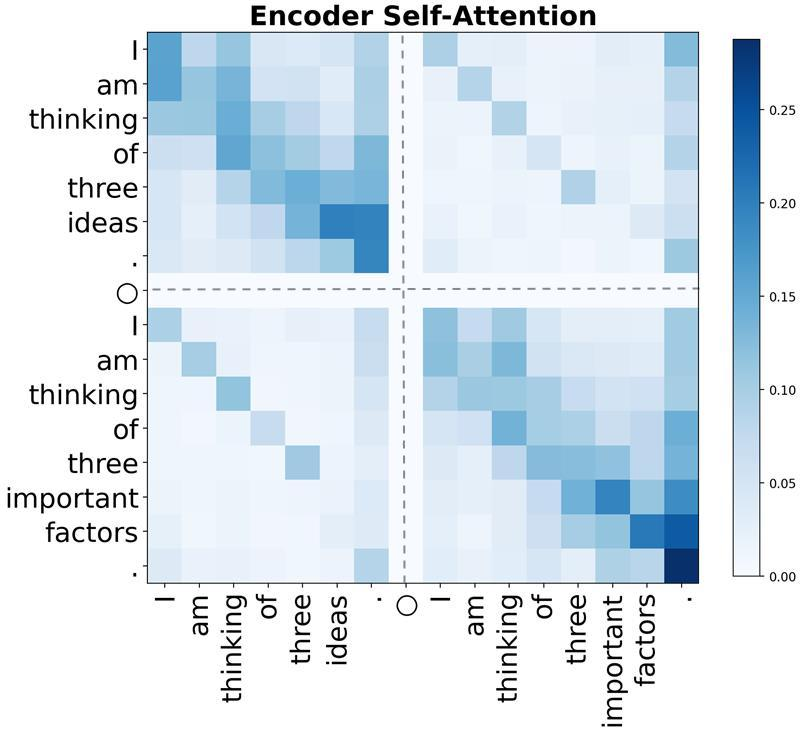
\includegraphics[width=.92\linewidth]{graphics/attention_enc.png}
    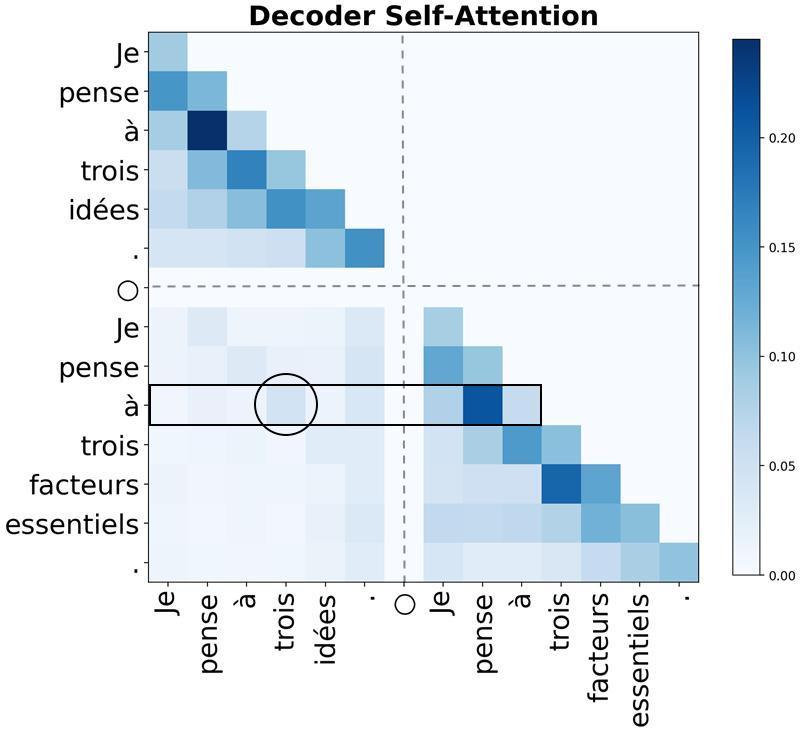
\includegraphics[width=.92\linewidth]{graphics/attention_dec.png}
\caption{Average attention values of all heads through all layers for the encoder (top) and decoder (bottom). Dashed lines are used to separate similar and input sentences.}
\label{fig:attn-chap8}
\end{figure}

Figure \ref{fig:attn-chap8} displays the attention\footnote{We use the average of all heads through all layers.} values for sentence $s=$ [{\bf I am thinking of three important factors .}] when translated into $t=$ [{\bf Je pense à trois facteurs essentiels .}] using the similar translation example $s^1=$ [{\it I am thinking of three ideas .}] and $t^1=$ [\textcolor{blue}{{\it Je pense à trois idées .}}]. For visualization purposes we mask the attention of the sentence separator token $\circ$.

Concerning the encoder self-attention (top), we can clearly observe that the encoder pays attention to the words in the similar sentence (down-left) when embedding the input sentence (down-right). 
%
Equivalently, the decoder self-attention (bottom) also attends to the similar translation (down-left: prefix words generated in forced mode) when producing the translation of sentence $s$. Note that when the decoder is about to generate the French word {\it trois [three]}, attention weights (rectangle) are the highest for the preceding words (in particular to {\it pense [think]}), with {\it trois} (circle in the similar translation) also receiving a substantial weight.
This suggests that the model has learned to use similar translations passed in the form of a target prefix to help generating translations.

\subsection*{Priming Model} 
The priming network leverages similar sentences from a TM so as to yield more accurate translations. From a mathematical perspective, the search for the best translation $\Bar{t}$ is conditioned to the input sentence $s$ as well as to similar pairs of translations $s^1$ and $t^1$:\fyDone{also condition on s?}
\begin{equation*}
    \Bar{t} = \mathop{\argmax}_{t}P(t|s,s^1,t^1)
\end{equation*}
\noindent to facilitate reading we use one single similar translation ($s^1$ and $t^1$) rather than $k$-best translations.

To evaluate the intuition that $P(t|s, s^1,t^1)$\fyDone{conditional probability} gives better translations than $P(t|s)$, we report the average of $\log P(t|s,s^1,t^1)$ computed by \system{CBON s+t$^5$} and of $\log P(t|s)$ computed by \system{Base} over test sets sentences with similar sentences translations.

Table~\ref{tab:probabilities-chap8} reports the difference between the token average of $\log P(t|s,s^1,t^1)$ and the token average of $\log P(t|s)$. More precisely, for each test sentence $s$, we compute the log probability of predicting reference $t$, we then sum all the calculated log probabilities and divide the sum by the total number of tokens in the references. For each test set, we computed the average log probability of model \system{CBON s+t$^5$} and \system{Base}. We report the difference in the average of both models. 
%of model \system{CBON s+t$^5$} and model \system{Base}.
Results indicate that $\log P_{\system{CBON s+t$^5$}}(t|s^1,s,t^1)$ are actually greater than $\log P_{\system{Base}}(t|s)$ in most cases, with the exception of \domain{EPPS} and \domain{NEWS} for which the base system yields higher probabilities. We observe a strong correlation between values reported and the gap in \texttt{BLEU} score for the same model configurations.\fyDone{for the same model?}

\begin{table}[h!]
\begin{center}
\scalebox{1.0}{
  \begin{tabular}{|l|c|}
    \hline
    Domain        & \system{CBON s+t$^5$} $-$ \system{Base} \\
    \hline
    \domain{ECB}  & 0.222 \\
    \domain{EMEA} & 0.231 \\
    \domain{EPPS} & \textcolor{red}{-0.039} \\
    \domain{GNOME}& 0.248 \\
    \domain{JRC}  & 0.165 \\
    \domain{KDE4} & 0.252 \\
    \domain{NEWS} & \textcolor{red}{-0.173} \\
    \domain{WIKI} & 0.009 \\
    \hline
  \end{tabular}
  }
\end{center}
  \caption{Differences of token average log probability between \system{CBON s+t$^5$} and \system{Base} model.}
  \label{tab:probabilities-chap8}
\end{table}

\subsection*{Similarity over Synthetic Sentences}

Results in Table~\ref{tab:results2-chap8} show a clear boost in performance ($\sim$2 \texttt{BLEU} points) when making use of synthetic translations of the \domain{WIKI} monolingual data set.
We now want to measure the noise introduced by synthetic translations when compared to human translations.
Thus, we consider the input sentences of the \domain{WIKI} test set for which we found similar sentences in both the parallel (human translation) and monolingual (synthetic translation) corpus (279 sentences).

Results in Table \ref{tab:bt-chap8} show a clear drop in \texttt{BLEU} scores when using synthetic matches.
As expected, machine translation quality degrades the results of similarity search which in turns provides less valuable similar translations.\fyFuture{We need translations, or just the results of encoding?}

\begin{table}[h!]
\begin{center}
\scalebox{1.0}{
  \begin{tabular}{|l|c|}
    \hline
    Priming sentences & \domain{WIKI} \\
    \hline
    par (human)    & 52.50 \\
    mon (synthetic)   & 49.94 \\
    \hline
  \end{tabular}
  }
\end{center}
  \caption{Results for a reduced test set (279 sentences) using \system{CBON} when priming with human and synthetic (back-translated) translations.}
  \label{tab:bt-chap8}
\end{table}

\section{Related Work}
\label{sec:related-chap8}

Our work relates to the ideas introduced in \citet{bulte19neural} and \citet{xu20boosting}.
Both of them leverage similar translations from parallel corpora and inject similar sentences in the NMT network.
While \citet{bulte19neural} integrates fuzzy matches into the NMT model by concatenating similar translations to source sentences, \citet{xu20boosting} extended the framework by adding additional source side features to distinguish between related and unrelated words, employed distributed sentence representations.
A similar idea is also explored in \citet{schwenk2019ccmatrix}, where the authors use multilingual sentence embeddings to retrieve pairs of similar sentences and train models uniquely with such sentences.

Previously, \citet{Niehues16pretranslation} augmented input sentences with pre-translations generated by a phrase-based MT system.
Our work, in contrast, integrates similar sentences in both source and target sides and employs similar translations found in parallel as well as monolingual data sets. 

A similar strategy of concatenating previous and current sentences was explored by \citet{tiedemann17neural} further evaluated by \citet{bawden18evaluating}
in the context of tackling discourse phenomena. 
Our work employs force decoding to allow including true translations in the decoder target-side.
Thus, avoiding the error propagation problem~\cite{Ranzato15sequence} of longer sequences in auto-regressive models.

~\citet{bapna19non} propose a neural MT model that incorporates
retrieved neighbours relying on local phrase level similarities.
%
Using deep pre-trained models \cite{peters18deep,radford19language,Devlin19bert,Conneau19crosslingual} to compute contextualized sentence representations has become common fashion in recent works \cite{feng20languageagnostic,chang20pretraining}.
However, deep models suffer from computation complexity when applied on-the-fly for inference.
We propose an extension of \texttt{sent2vec} \cite{pagliardini18unsupervised} to compute sentence representations that also inherits from the computationally efficient bilinear models~\cite{Mikolov13efficient,Mikolov13distributed,Pennington14glove}. 

Similar to our work, \citet{Farajian17multidomain} and \citet{Li18onesentence} retrieve similar sentence to dynamically adapt each individual input sentence. 
\citet{Farajian17multidomain} obtains best performance when tuning the adaptation learning rate and number of epochs according to level of similarity between the input and retrieved sentences.
In~\citet{xu19lexical} the model is dynamically adapted to a entire test set to reduce adaptation time.
\fyDone{One more word on Farajian to explain adaptive epoch et}

In computer vision, priming network has been recently studied. For the object detection task , \citet{Rosenfeld18Priming} primed the network via an external information that affects all the processing layers. Upon processing each image in the network, \citet{Rosenfeld18Priming} also presented the network with the category of the object in the image; this information is injected at all layers. \fyDone{Style}

\section{Conclusions and outlook}
\label{sec:conclusions-chap8}
We presented a novel method that injects similar translations in the NMT network as prefixes of the decoder. The proposed method obtains higher translation accuracy results and reduces the undesirable effect observed in previous methods of copying unrelated words when performing translations. 

We evaluate results on a multi-domain setting using a single model trained on a heterogeneous data set, built from multiple corpora and domains, achieving better results when compared to previous micro-adaptation approaches. In addition, we showed the suitability of our approach to gather valuable information from large monolingual corpora. 

In our future work, we would like to explore alternative algorithms to compute distributed sentence representations from word embeddings, such as TF-IDF. Furthermore, we would like to consider source sentence coverage when selecting $n$-best similar translations. As regards distributed representations we plan to experiment with cross-lingual networks to retrieve similar translations directly from human-crafted monolingual data in order to eliminate the noise introduced by synthetic translations.
